% CREATED BY DAVID FRISK, 2016
% MODIFIED BY ALEXANDER HÅKANSSON, 2017

% COVER PAGE
\begin{titlepage}
\newgeometry{top=3cm, bottom=3cm,
			left=2.25 cm, right=2.25cm}	% Temporarily change margins		
			
% Cover page background 
\AddToShipoutPicture*{\backgroundpic{-4}{56.7}{figure/front/frontpage-en-GU.pdf}}
\addtolength{\voffset}{2cm}

% Cover picture (replace with your own or delete)		
\begin{figure}[H]
\centering
\vspace{1cm}	% Adjust vertical spacing here
%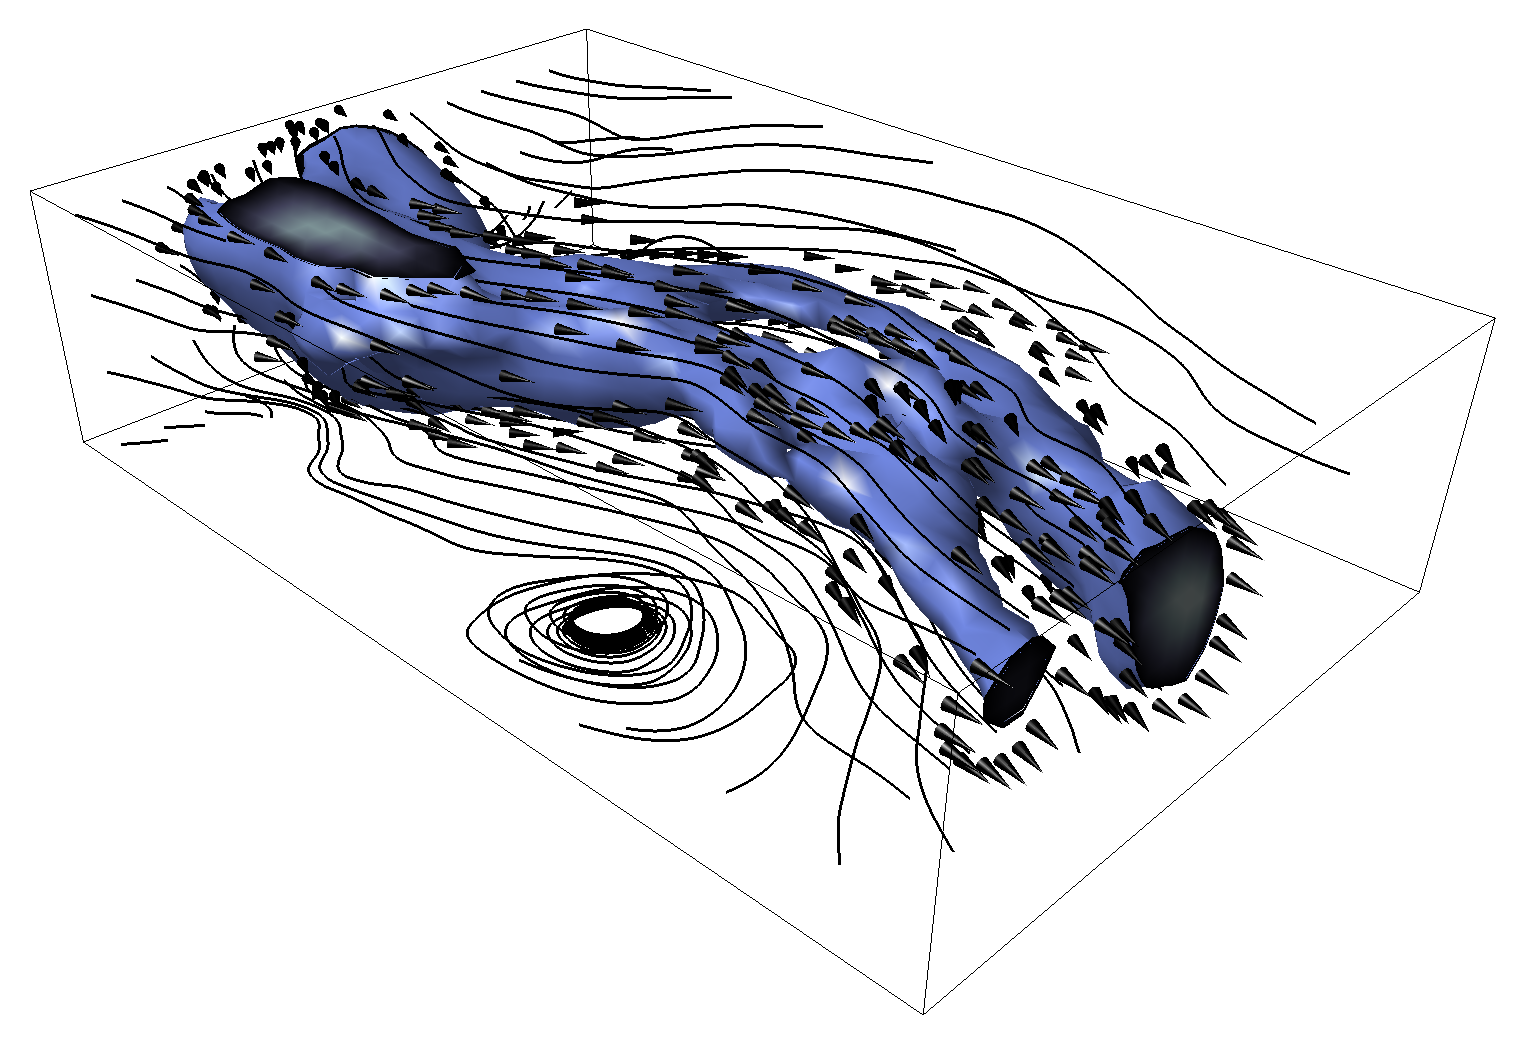
\includegraphics[width=0.9\linewidth]{figure/Wind.png}
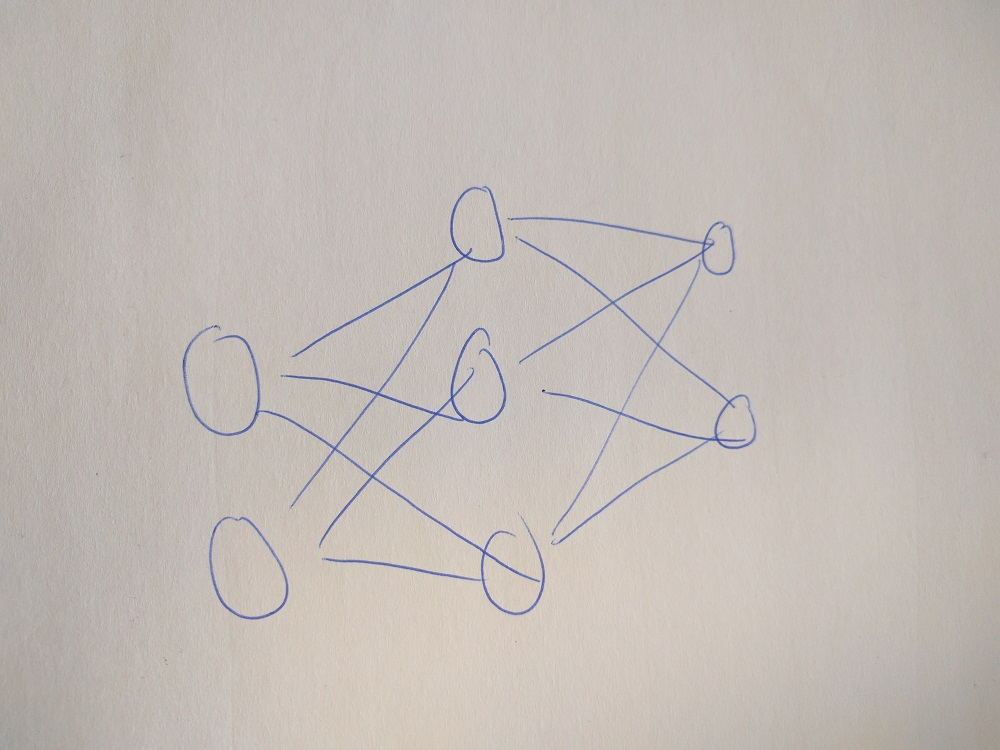
\includegraphics[width=0.9\linewidth]{figure/ann/ann}
\end{figure}

% Cover text
\mbox{}
%\vfill
\renewcommand{\familydefault}{\sfdefault} \normalfont % Set cover page font
\begin{flushleft}
\textbf{{\Huge \varthetitle}} 	\\[0.5cm]
{\LARGE \varthesubtitle}\\[0.2cm]
Bachelor of Science Thesis in Computer Science and Engineering \setlength{\parskip}{0.5cm}

{ JESPER JAXING, ALEXANDER HÅKANSSON, MAXIM GORETSKYY, GMAL TCHAEFA, AXEL OLIVECRONA, JONATAN ALMÉN} \setlength{\parskip}{1.9cm}\\
\vfill
Chalmers University of Technology \\
University of Gothenburg \\
Department of Computer Science and Engineering \\
Göteborg, Sweden, June 2017

\end{flushleft}
%\renewcommand{\familydefault}{\rmdefault} \normalfont % Reset standard font
\end{titlepage}

%\begin{comment} % Remove comment to get blank page
% BACK OF COVER PAGE (BLANK PAGE)
\newpage
\restoregeometry
\thispagestyle{empty}
\mbox{}
%\end{comment}

% TITLE PAGE
\newpage
\setcounter{page}{1}
\thispagestyle{empty}
\begin{center}
	\large Bachelor of Science Thesis\\[4cm]		% Report number given by department 
	\textbf{\large \varthetitle} \\[0.7cm]
	{\large \varthesubtitle}\\[1cm]
	{\large JESPER JAXING}\\
	{\large ALEXANDER HÅKANSSON} \\
	{\large MAXIM GORETSKYY} \\
	{\large GMAL TCHAEFA } \\
	{\large AXEL OLIVECRONA} \\
	{\large JONATAN ALMÉN} \
	
	\vfill	
	% Logotype on titlepage	
	\begin{figure}[H]
	\centering
	% Remove the following line to remove the titlepage logotype
	%
\includegraphics[width=0.2\pdfpagewidth]{figure/front/logo_eng.pdf} \\	
	\end{figure}	\vspace{5mm}	
	
	Department of Computer Science and Engineering \\
	CHALMERS UNIVERSITY OF TECHNOLOGY \\
	University of Gothenburg \\[0.5cm]
	Göteborg, Sweden 2017 \\
\end{center}


% IMPRINT PAGE (BACK OF TITLE PAGE)
\newpage
\thispagestyle{plain}
%\vspace*{4.5cm}
\textbf{\varthetitle}\\
\varthesubtitle
\vspace*{0.5cm}\\
JESPER JAXING\\
ALEXANDER HÅKANSSON\\
MAXIM GORETSKYY\\
GMAL TCHAEFA\\
AXEL OLIVECRONA\\
JONATAN ALMÉN\setlength{\parskip}{0.7cm}

\copyright ~ JESPER JAXING, 2017\\
\copyright ~ ALEXANDER HÅKANSSON, 2017\\
\copyright ~ MAXIM GORETSKYY, 2017\\
\copyright ~ GMAL TCHAEFA, 2017\\
\copyright ~ AXEL OLIVECRONA, 2017\\
\copyright ~ JONATAN ALMÉN, 2017 \setlength{\parskip}{0.5cm}

\todo{Dubbelkolla så detta stämmer}
Examiner: Richard Johansson, Department of Computer Science and Engineering \setlength{\parskip}{1cm}

Department of Computer Science and Engineering\\
Chalmers University of Technology\\
University of Gotehnburg\\
SE-412 96 Göteborg\\
Sweden\\
Telephone: +46 (0)31 772 1000 \setlength{\parskip}{0.5cm}

\vfill
The Authors grants to Chalmers University of Technology and University of Gothenburg the non-exclusive right to publish the Work electronically and in a non-commercial purpose make it accessible on the Internet.\\\\
The Author warrants that he/she is the author to the Work, and warrants that the Work does not contain text, pictures or other material that violates copyright law.\\\\
The Author shall, when transferring the rights of the Work to a third party (for example a publisher or a company), acknowledge the third party about this agreement. If the Author has signed a copyright agreement with a third party regarding the Work, the Author warrants hereby that he/she has obtained any necessary permission from this third party to let Chalmers University of Technology and University of Gothenburg  store the Work electronically and make it accessible on the Internet.


\vfill
% Caption for cover page figure if used, possibly with reference to further information in the report
Cover:\\
A graph visualisation of a simple artificial neural network. See Chapter \ref{chap:ann} for more details. \setlength{\parskip}{0.5cm}

Department of Computer Science and Engineering\\
Göteborg, Sweden 2017

